\begin{figure}
  \centering
  \begin{subfigure}[t]{0.95\textwidth}
    \centering
    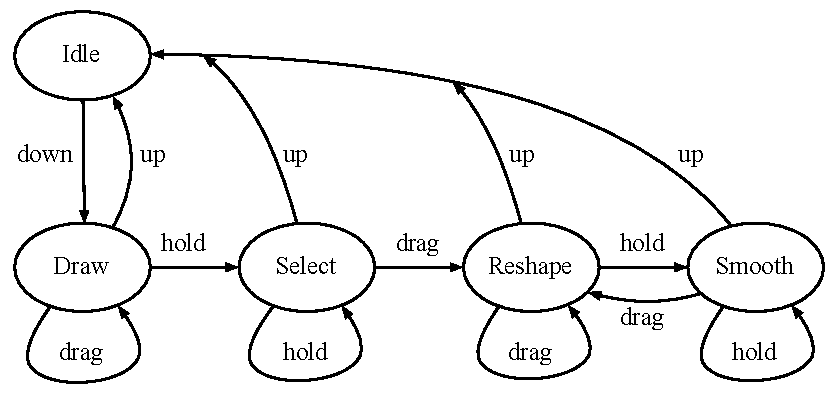
\includegraphics[width=0.5\linewidth]{img/flow-selection-fsm.pdf}
    \caption{Finite state machine that models flow
    selection. Most of the time, users simply press the pen down, draw
    some ink, and release. But if they hold the pen down, the flow
    selection states are reached. The user holds down the pen to
    select a region, moves the pen to move the selection, and holds it
    still once again to smooth the selection. Lifing the pen ends the
    process.}
    \label{fig:flow-selection-fsm}
  \end{subfigure}
  
  \vspace{5mm}
  \begin{subfigure}[t]{0.95\textwidth}
    \centering
    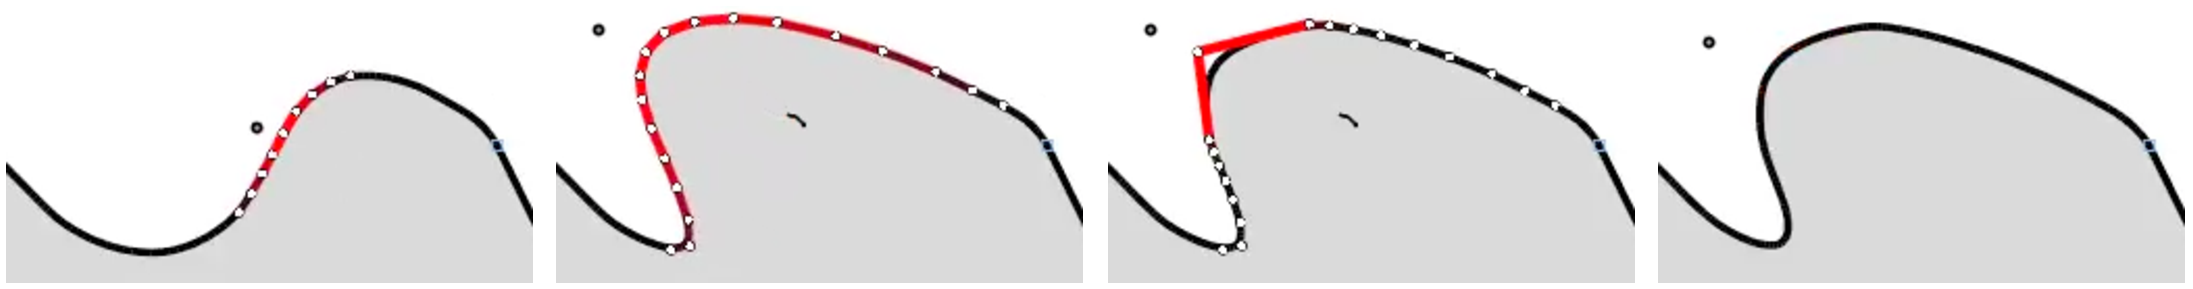
\includegraphics[width=\linewidth]{img/flow-selection-example.pdf}
    \caption{Example showing the user deforming a curved segment. The
      user holds the pen to heat a region, and moves the stylus to
      move that region. Next the user dwells to smooth region. The
      final state is at right.}
    \label{fig:flow-selection-example}
  \end{subfigure}
  \caption[Flow Selection]{Interaction and implementation of Flow Selection.}
  \label{fig:flow-selection}
\end{figure}
